Po analýze tvorby dokumentů a nástrojů na vytváření dokumentů je na čase připravit návrh aplikace, která bude řešit správu, vytváření a verzování
modulárních dokumentů. Tato kapitola bude rozdělena do jednotlivých sekcích, ve kterých budeme podrobně popisovat návrh dané sekce v naší aplikaci.
V rámci návrhu nesmíme opomenout ani možnosti budoucího rozšíření.

\section{Užitelská sekce}

Tato sekce je zde hlavně pro potřeby vytváření neveřejných dokumentů, které nesmí být přístupné veřejnosti. Dále je také potřeba vytvořit možnost
správy systému, která bude jednoduchá na použítí a nebude nutné například zasahovat přímo do databáze naší aplikace. Pro tuto funkcionalitu bude ovšem
nutné vytvořit speciální roli, která bude tohoto administrátora jasně identifikovat. Role ale nebude pouze administrátorská, všichni uživatelé budou mít
možnost být nositeli až několika rolí zároveň. Tato vlastnost je zde kvůli jednodušší obsluze přiřazování oprávnění k dokumentům a repozitářům, které si rozebereme
dále v textu. Aby hlavní administrátor aplikace nemusel tyto požadavky na přidělení rolí řešit on sám, bude zde ještě další pevně definovaná role a to role
správce přístupu, který bude mít možnost, stejně jako administrátor, hromadně přidělovat či odebírat role. Ovšem pouze administrátor může přiřadit roli správce přístupu.

Nyní si probereme vlastnosti uživatele, budeme potřebovat uživatele jednoznačně identifikovat, je tedy potřeba od uživatele získat nějaký údaj, který bude unikátní
jako například uživatelské jméno, dále si od uživatele vyžádáme ještě email, který může být posléze použit k doručení zpráv a upozornění z aplikace. Tímto se ovšem
dostáváme k nutnosti myslet na ochranu osobních údajů, která prošla v posledních letech změnou v důsledky nabití účinosti evropského nařízení \gls{gdpr}.

V tomto UC diagramu \ref{fig:userUCDiagram} naleznete rozpis všech UC, které se týkají uživatelské sekce. Zároveň k tomu je zde také stavový diagram \ref{fig:userFlow},
který nám ukazuje jednotlivé stavy uživatele, vzhledem k systému a které akce mají vliv na jeho stav.

\subsection{\gls{gdpr}}

Naše aplikace bude pracovat s osobními údaji, je nutné toto brát na~vědomí, proto se nyní podívejme na to, co musí naše aplikace splňovat, aby dodržela všechny
zákony o ochraně osobních údají a směrnice Evropské unie, \gls{gdpr}. První co je nutné brát na vědomí je účel, za kterým údaje chceme údaje sbírat a uchovávat a jestli je náš
účel oprávněný. V tomto případě o uživateli získáme osobní údaj v podobě emailu, který stačí k identifikaci určité osoby. V našem případě je email identifikátor uživatele
a budeme jej při registraci žádat o souhlas se zpracováním osobních údajů. Dále musíme myslet na možnost smazání či anonymizace údajů uživatele. Toho docílíme ručními
zásahy do databáze, kde využijeme možnosti změnit email na jeho hash. \cite{gdpr}

\section{Repozitáře}

Než začneme popisovat samotné generování dokumentů, je potřeba si \mbox{definovat} repozitáře našich modulů. Jednotlivé repozitáře nám budou sloužit jako složky,
které budou obsahovat moduly, ze kterých se pak budou skládat výsledné dokumenty. V rámci repozitářů je potřeba hlavně zajistit správně fungování oprávnění.
Pokud si uživatel založí nový repozitář, má vůči němu všechny práva, ostatní uživatelé se o tomto repozitáři v tomto stavu nemají jak\linebreak dozvědět, je pro ně
skrytý. Pokud se ovšem zakladatel rozhodne svůj obsah repozitáře sdílet, má možnost sdílet repozitář s jednotlivými uživateli, uživatelskými rolemi a nebo
změnit repozitář na veřejný. Dále má také možnost definovat, jestli je repozitář pro jednotlivé uživatele pouze pro čtení, či použití modulu v dokumenty,
nebo jestli je možnost moduly i upravovat.

V neposlední řadě musíme myslet na verzování našich jednotlivých modulů, zde se nabízejí 2 možnosti jak tomuto přistoupit, buď by bylo možné integrovat
řešení založené na nějaké \gls{vcs}, jedná se systém, který zařizuje verzování souborů,
nebo je možné implementovat verzování pomocí databáze. V této práci budeme volit verzování pomocí databáze a to hlavně z časových důvodů, neboť
pro použití vcs by bylo nutné udělat kompletní obal na nějaký již existující verzovací systém. Na digramu \ref{fig:moduleDia} je vidět jak by měly
vypadat vztahy mezi jednotlivými moduly.
\todo{uc pro repozitáře a dokumenty}
\subsection{Přehled všech příkladů užití}

V repozitářích máme 2 hlavní části na které se musíme zaměřit, tou první je nutnost hlídat oprávnění a také je mít možnost spravovat. Tudíž majitel
repozitáře musí mít možnost ovlivňovat, kdo má, či nemá, přístup do jeho repozitáře. Dále musí mít možnost prohlásit svůj repozitář za veřejný a tím
dát možnost všem uživatelům do něj vstoupit. Krom oprávnění je potřeba také zajistit vytváření nových modulů a verzování jejich úprav. U verzování je
potřeba si pamatovat kdo a kdy vytvořil novou verzi. A také možnost vrátit se k určité předchozí verzi.

\section{Dokumenty}

Jelikož už máme definované chování pro jednotlivé repozitáře a jejich moduly, můžeme se vrhnout na návrh dokumentů, které se budou skládat z modulů. Každý
dokument je tedy soubor modulů, který je možné převést do tisknutelné podoby. Na co ale nesmíme zapomenout, že stejně jako moduly bude možné dokumenty také
verzovat, zde to bude provedeno pomocí revizí. Každá revize bude nést informace o tom, kdo danou revizi vytvořil a také ponese všechny informace o verzích
modulu, které jsou na danou revizi použity.

Podobně jako u repozitářů i u dokumentů budeme řešit oprávnění a to stejným způsobem, tudíž každý dokument má svého zakladatele nebo také vlastníka,
vlastník má možnost rozhodovat o tom, kdo bude moci dokument upravovat (vytvářet nové revize, měnit obsah dokumentu), a kdo bude mít možnost si pouze dokument
přečíst. Dále také bude možnost prohlásit dokument za veřejný a bude tedy přístupný všem uživatelům.

\subsection{Příklady užití v dokumentech}

Pro dokumenty bude důležité hlavně možnost jejich generovaní do přenosného formátu, jakým je například \gls{pdf}. Dalším důležitou funkcionalitou bude možnost přiřazování
oprávnění jako je tomu u repozitářů, nesmí chybět ani možnost dokument prohlásit za veřejný a tím jej spřístupnit všem uživatelům. Je také potřeba myslet na možnost
procházet a generovat i starší revize.

\begin{figure}[H]
    \centering
    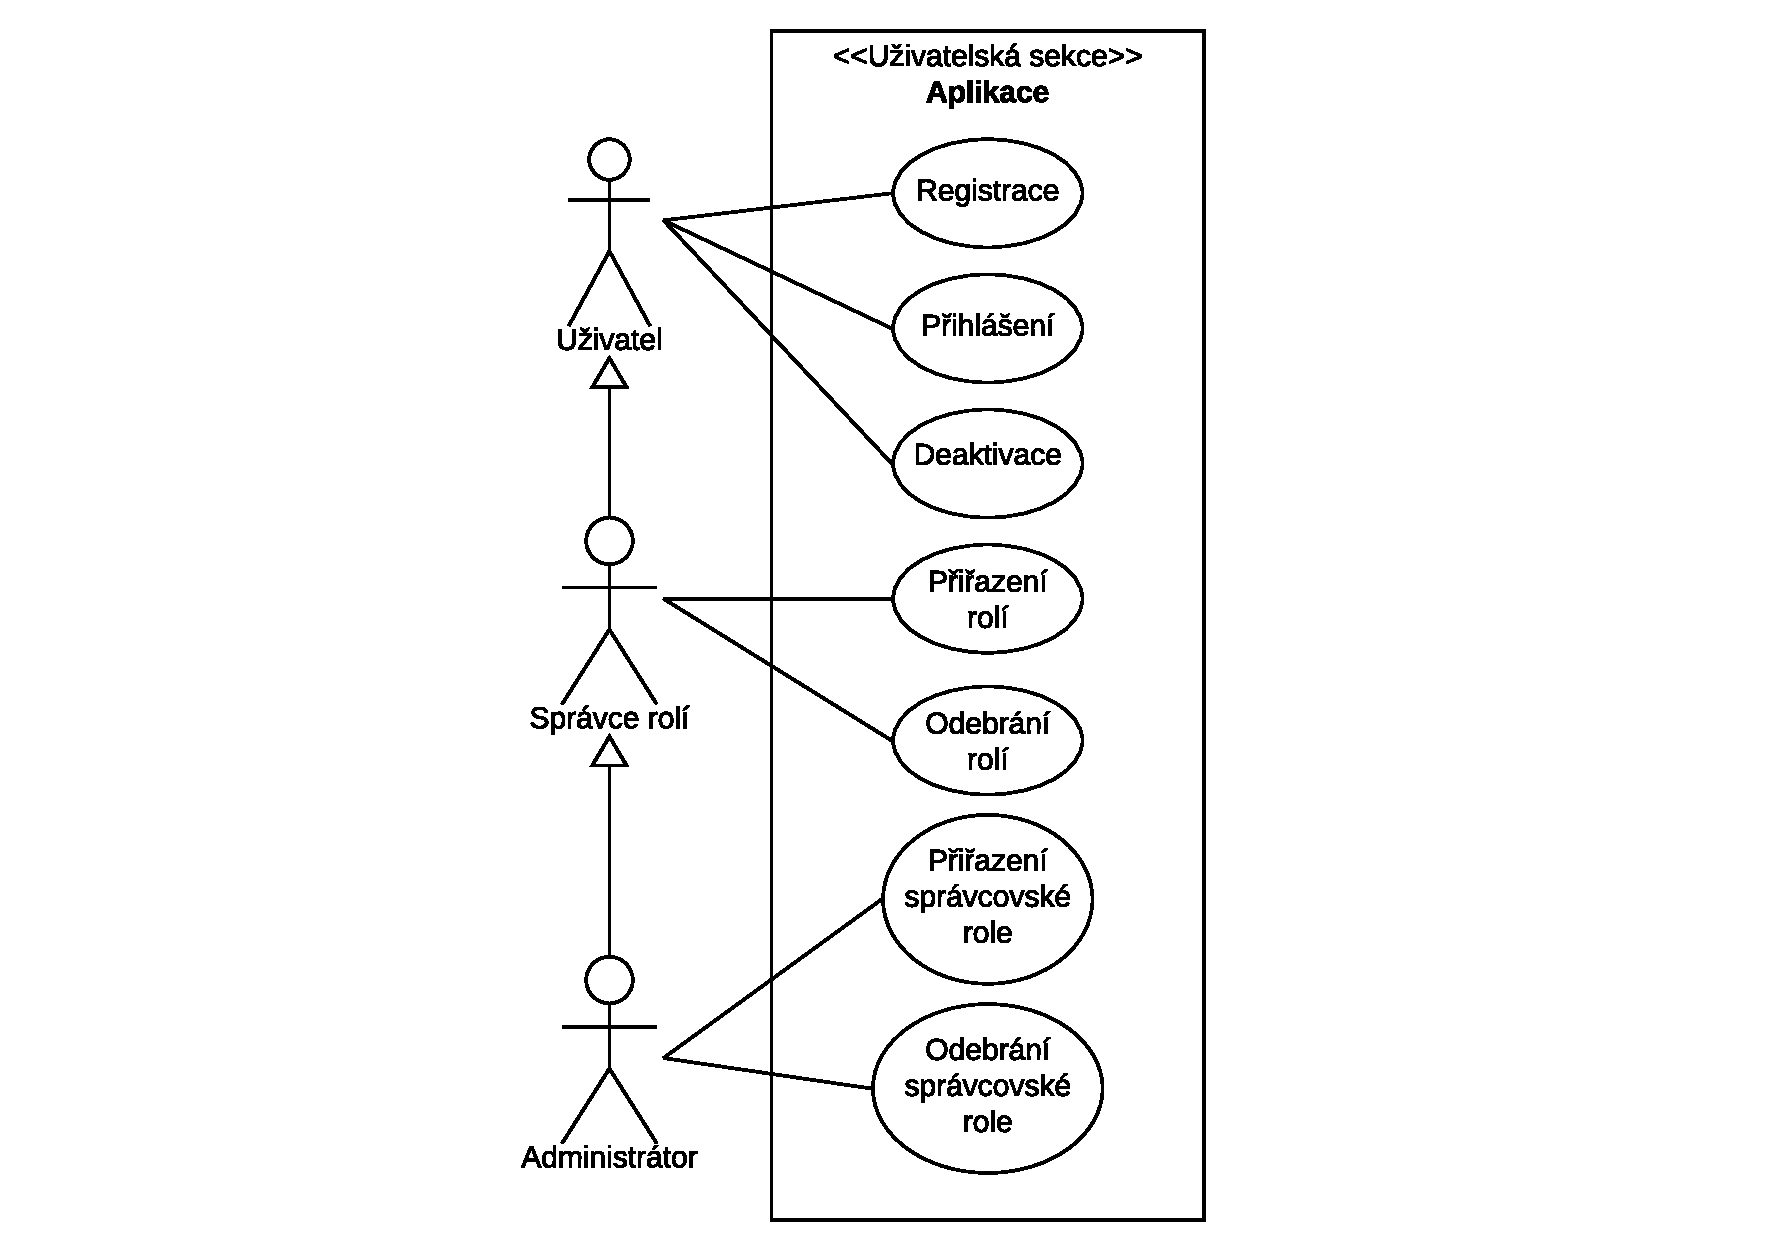
\includegraphics[width=\textwidth]{userUCDiagram.pdf}
    \caption{Diagram UC pro uživatelskou sekci}
    \label{fig:userUCDiagram}
\end{figure}

\begin{figure}[h]
    \centering
    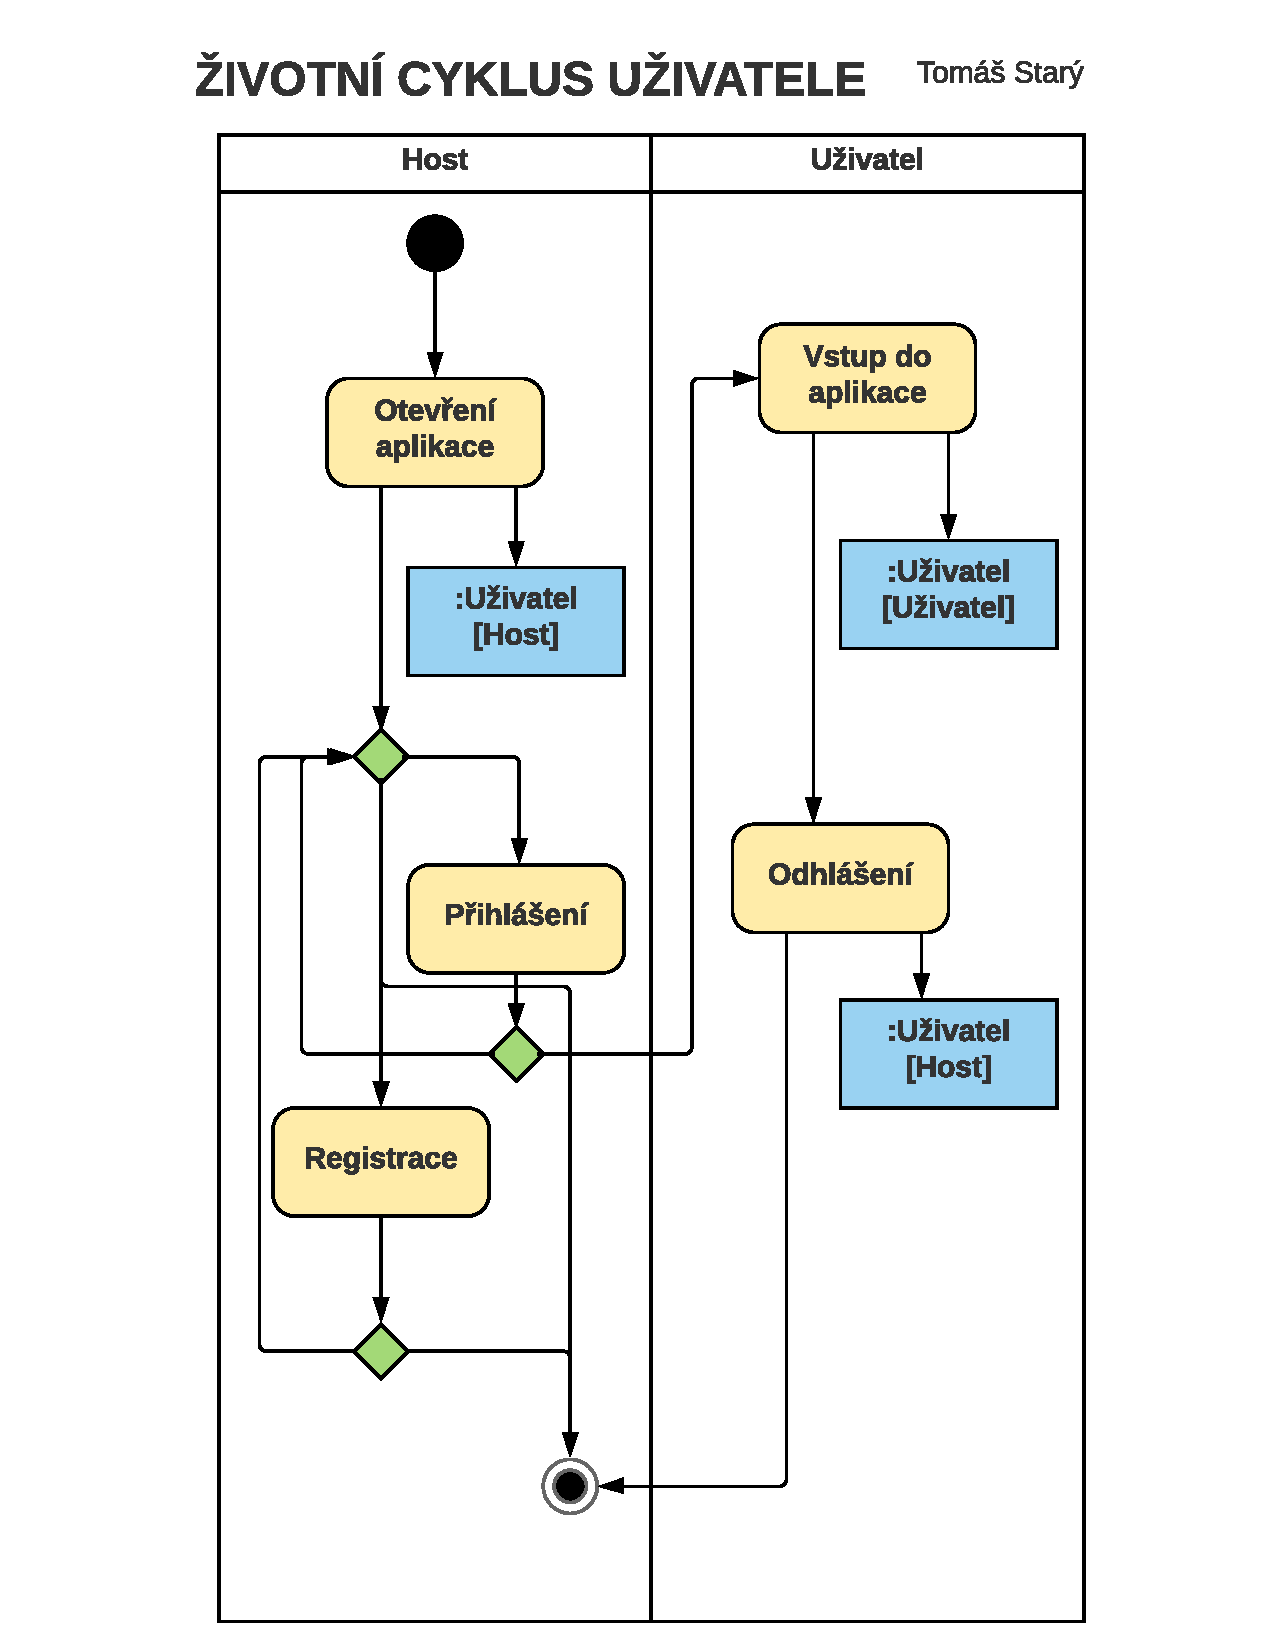
\includegraphics[width=\textwidth]{lifecycle.pdf}
    \caption{Diagram přihlášení a registrace uživatele}
    \label{fig:userFlow}
\end{figure}

\begin{figure}[h]
    \centering
    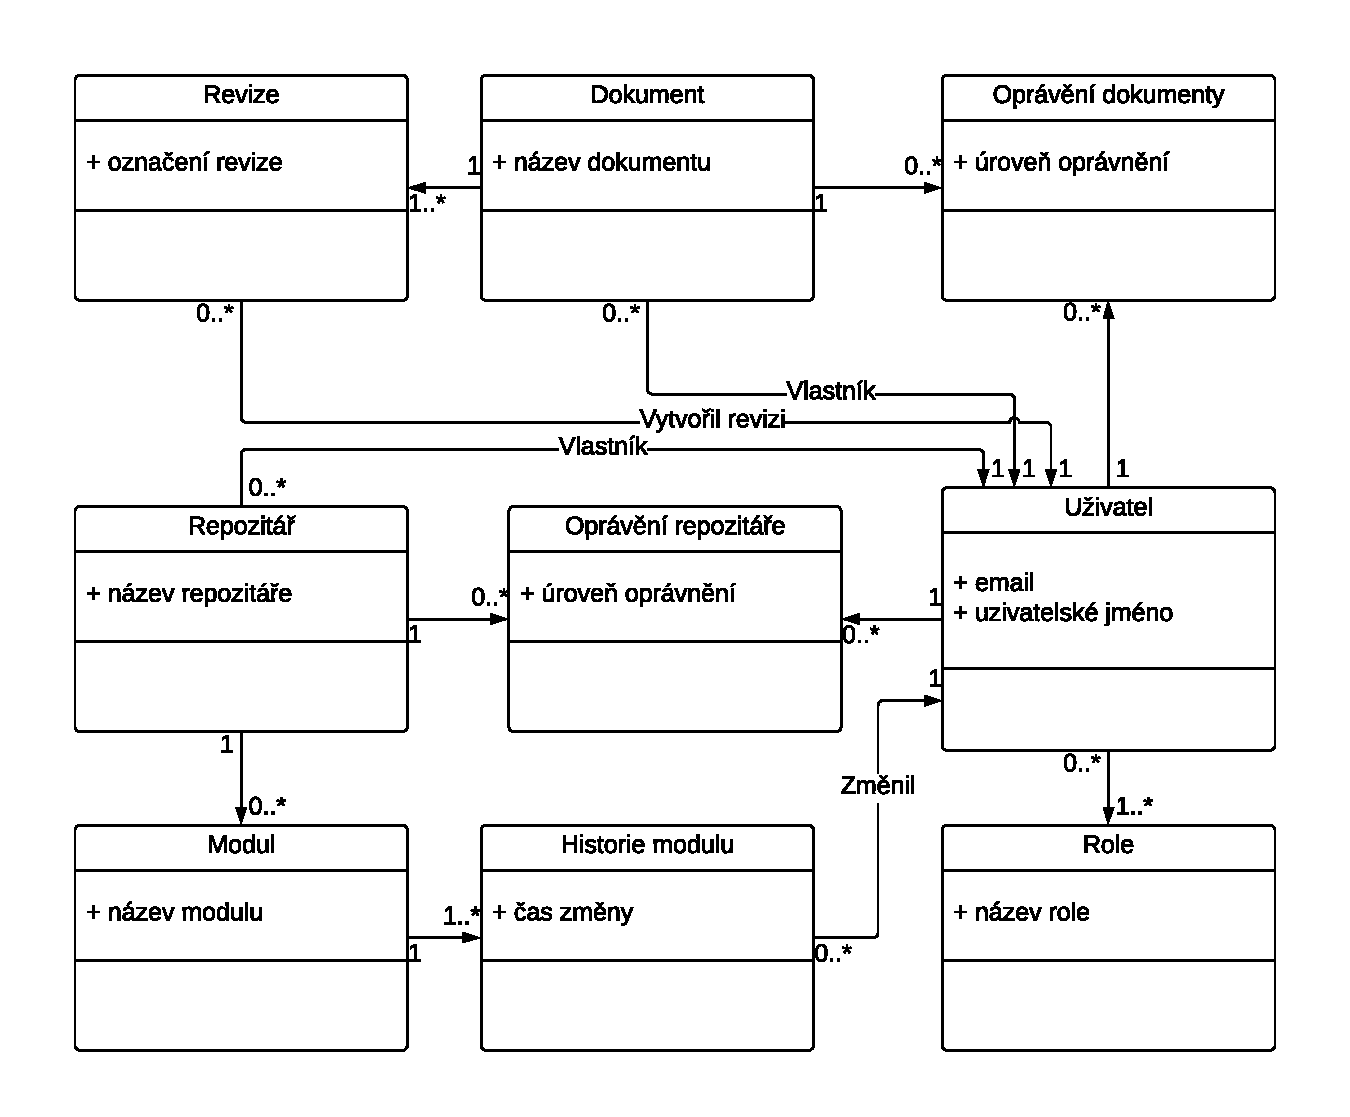
\includegraphics[width=\textwidth]{module_diagram.pdf}
    \caption{Návrh rozložení modelů}
    \label{fig:moduleDia}
\end{figure}